%%%%%%%%%%%%%%%%%%%%%%%%%%%%%%%%%%%%%%%%%%%%%%%%%%%%%%%%%%%%%%%%%%%%%%%%%%%%%%%%
\chapter{Обзор методов классификации и обнаружения транспортных средств с использованием методов технического зрения}
%%%%%%%%%%%%%%%%%%%%%%%%%%%%%%%%%%%%%%%%%%%%%%%%%%%%%%%%%%%%%%%%%%%%%%%%%%%%%%%%

%%%%%%%%%%%%%%%%%%%%%%%%%%%%%%%%%%%%%%%%%%%%%%%%%%%%%%%%%%%%%%%%%%%%%%%%%%%%%%%%
\section{Обнаружение транспортных средств по моделям (Model-Based Detection)}
%%%%%%%%%%%%%%%%%%%%%%%%%%%%%%%%%%%%%%%%%%%%%%%%%%%%%%%%%%%%%%%%%%%%%%%%%%%%%%%%

Обнаружение транспортных средств по модели осуществляется с использованием большой базы данных заранее подготовленных моделей. Во время работы этого метода, система пытается найти подходящую область в заданных кадрах пользуясь информацией из базы моделей. Для определения совпадения задается некоторый порог. Если результат сравнения между моделью и областью в кадре больше, чем заданный порог, тогда эта область будет определена как транспортное средство. Пример работы такого метода можно наблюдать на рисунке ниже.

\begin{figure}[htbp]
\centering
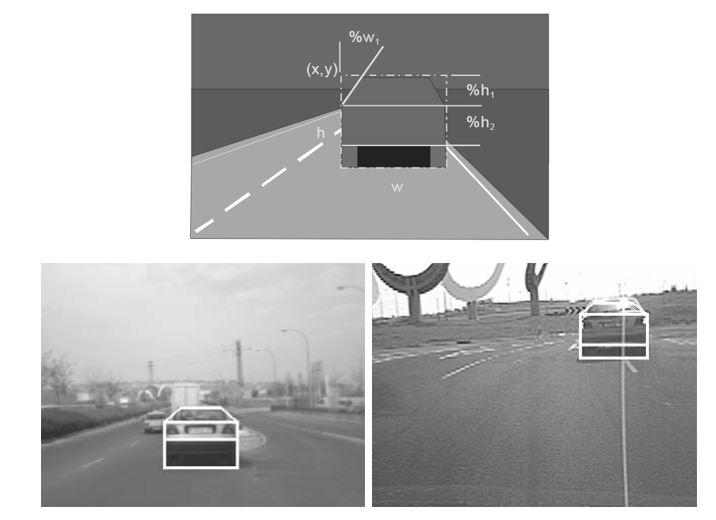
\includegraphics[width=0.5\textwidth]{image001.jpg}
\caption{Пример обнаружения по модели~\cite{one}}%
\label{fig:how-to-do-research}
\end{figure}

%%%%%%%%%%%%%%%%%%%%%%%%%%%%%%%%%%%%%%%%%%%%%%%%%%%%%%%%%%%%%%%%%%%%%%%%%%%%%%%%
\section{Обнаружение транспортных средств методами машинного обучения}
%%%%%%%%%%%%%%%%%%%%%%%%%%%%%%%%%%%%%%%%%%%%%%%%%%%%%%%%%%%%%%%%%%%%%%%%%%%%%%%%

Есть определенные особенности транспортных средств, которые позволяют отличить их от других объектов на изображении (грани, тени, симметрия). В ходе обнаружения, последовательно осуществляется поиск подобных характерных признаков на всем изображении. Минусы подобных алгоритмов заключаются в том, что если один из признаков отсутствует на изображении, то объект не может быть обнаружен. Также существует высокая вероятность ложного срабатывания.

В методах, основанных на классификаторах по признакам, транспортное средство рассматривается как единое целое. Процесс обнаружения заключается в выделении области, в которой находится транспортное средство. Для каждого кадра производится разделение изображения на несколько регионов. Процесс разделения определяется размером искомых признаков. После выполнения деления, выполняется извлечение признаков из каждого региона (гистограмма направленных градиентов ~(HOG), признаки Хаара, локальные бинарные оттенки ~(LBP)). Для выполнения классификации по признакам используются специальные классификаторы. Для использования этого метода необходимо правильно выбрать признаки, которые лучшим образом описывают транспортное средство. Из-за большого количества вариаций углов обзора это становится сложной задачей.
\nomenclature{HOG}{Histogram of Oriented Gradients}
\nomenclature{LBP}{Local binary patterns}

%%%%%%%%%%%%%%%%%%%%%%%%%%%%%%%%%%%%%%%%%%%%%%%%%%%%%%%%%%%%%%%%%%%%%%%%%%%%%%%%
\subsection{Способы извлечения признаков}
%%%%%%%%%%%%%%%%%%%%%%%%%%%%%%%%%%%%%%%%%%%%%%%%%%%%%%%%%%%%%%%%%%%%%%%%%%%%%%%%

%%%%%%%%%%%%%%%%%%%%%%%%%%%%%%%%%%%%%%%%%%%%%%%%%%%%%%%%%%%%%%%%%%%%%%%%%%%%%%%%
\subsubsection{Признаки Хаара}
%%%%%%%%%%%%%%%%%%%%%%%%%%%%%%%%%%%%%%%%%%%%%%%%%%%%%%%%%%%%%%%%%%%%%%%%%%%%%%%%

Признаки Хаара можно посчитать несколькими методами. Например, можно использовать горизонтальные и вертикальные прямоугольники или квадратный набор прямоугольников, что проиллюстрировано на рисунке ниже.

\begin{figure}[htbp]
\centering
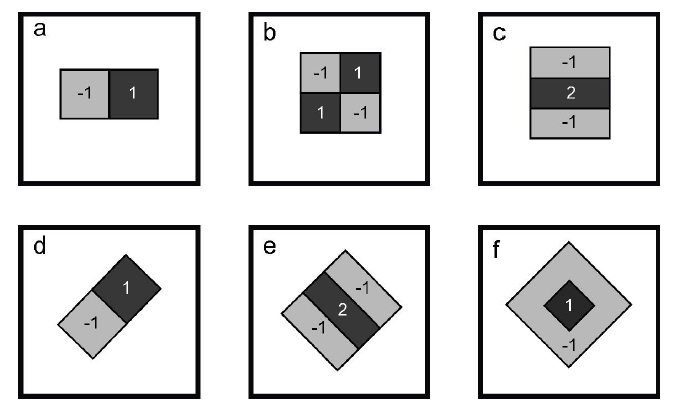
\includegraphics[width=0.5\textwidth]{image003.png}
\caption{Признаки Хаара~\cite{two}}%
\label{fig:how-to-do-research}
\end{figure}

Простейший прямоугольный признак Хаара можно определить~\cite{two}, как разность сумм пикселей двух смежных областей внутри прямоугольника, который может занимать различные положения и масштабы на изображении. Такой вид признаков называется 2-прямоугольным. Виола и Джонс~\cite{three} так же определили 3-прямоугольные и 4-прямоугольные признаки. Каждый признак может показать наличие (или отсутствие) какой-либо конкретной характеристики изображения, такой как границы или изменение текстур. Например, 2-прямоугольный признак может показать, где находится граница между темным и светлым регионами.

Линхарт и Майд~\cite{four} представили идею наклоненных (45$^{\circ}$ градусов) признаков Хаара. Это было сделано для увеличения размерности пространства признаков. Способ оказался удачным и некоторые наклонные признаки были способны лучше описывать объект. Например, 2-прямоугольный наклонный признак Хаара может показать наличие края, наклоненного на 45$^{\circ}$ градусов.

Мессом и Барзак~\cite{five} дополнили концепцию наклонных признаков Хаара. Хоть идея и является математически верной, на практике при использовании признаков под разными углами возникают проблемы. Для ускорения вычислений, алгоритм обнаружения использует изображения низкого разрешения, что приводит к ошибке округления. Исходя из этого, наклонные признаки Хаара обычно не используются.

%%%%%%%%%%%%%%%%%%%%%%%%%%%%%%%%%%%%%%%%%%%%%%%%%%%%%%%%%%%%%%%%%%%%%%%%%%%%%%%%
\subsubsection{Локальные бинарные оттенки (Local binary patterns)}
%%%%%%%%%%%%%%%%%%%%%%%%%%%%%%%%%%%%%%%%%%%%%%%%%%%%%%%%%%%%%%%%%%%%%%%%%%%%%%%%

Расчет признаков LBP происходит на сетке пикселей изображения. Значение каждого пикселя вокруг центрального сравнивается со значением центрального и заменяется либо единицей, либо нулем в зависимости от результата сравнения. После этого, как показано на рисунке ниже, все пиксели складываются с некоторыми коэффициентами и получается число. Разряды полученного числа описывают направления изменения яркости в изображении.

\begin{figure}[htbp]
\centering
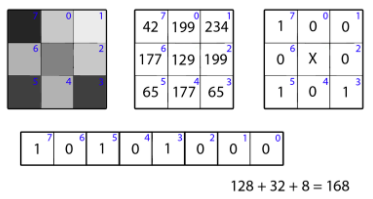
\includegraphics[width=0.5\textwidth]{image004.png}
\caption{Иллюстрация извлечения LBP признаков~\cite{six}}%
\label{fig:how-to-do-research}
\end{figure}

%%%%%%%%%%%%%%%%%%%%%%%%%%%%%%%%%%%%%%%%%%%%%%%%%%%%%%%%%%%%%%%%%%%%%%%%%%%%%%%%
\subsubsection{Гистограмма направленных градиентов (Histogram of Oriented Gradients)}
%%%%%%%%%%%%%%%%%%%%%%%%%%%%%%%%%%%%%%%%%%%%%%%%%%%%%%%%%%%%%%%%%%%%%%%%%%%%%%%%

Извлечение HOG признаков можно разделить на несколько шагов~\cite{seven}. Первым шагом вычислений во многих алгоритмах обнаружения особых точек является нормализация цвета и гамма-коррекция. На следующем шаге вычисляются гистограммы ячеек. Каждый пиксел в ячейке участвует во взвешенном голосовании для каналов гистограммы направлений, основанном на значении градиентов. Ячейки могут быть прямоугольной или круглой формы, каналы гистограммы равномерно распределяются от 0 до 180$^{\circ}$ или же от 0 до 360$^{\circ}$, в зависимости от того, вычисляется «знаковый» или «беззнаковый градиент». Далал и Триггс обнаружили, что беззнаковый градиент совместно с девятью каналами гистограммы дает лучшие результаты при распознавании людей. При распределении весов в голосовании вес пикселя может задаваться либо абсолютным значением градиента, либо некоторой функцией от него; в реальных тестах абсолютное значение градиента дает лучшие результаты. Другими возможными вариантами могут быть квадратный корень, квадрат или урезанное абсолютное значение градиента.

Для принятия во внимание яркости и контрастности градиенты следует локально нормировать, для чего ячейки нужно сгруппировать в более крупные связные блоки. Дескриптор HOG, таким образом, является вектором компонент нормированных гистограмм ячеек из всех областей блока. Как правило, блоки перекрываются, то есть каждая ячейка входит более чем в один конечный дескриптор. Используются две основные геометрии блока: прямоугольные ~(R-HOG) и круглые ~(C-HOG). Как можно видеть на рисунке ниже, блоки R-HOG обычно являются квадратными сетками, характеризующимися тремя параметрами: количеством ячеек на блок, количеством пикселов на ячейку и количеством каналов на гистограмму ячейки.
\nomenclature{R-HOG}{Rectangle Histogram of Oriented Gradients}
\nomenclature{C-HOG}{Circular Histogram of Oriented Gradients}

\begin{figure}[htbp]
\centering
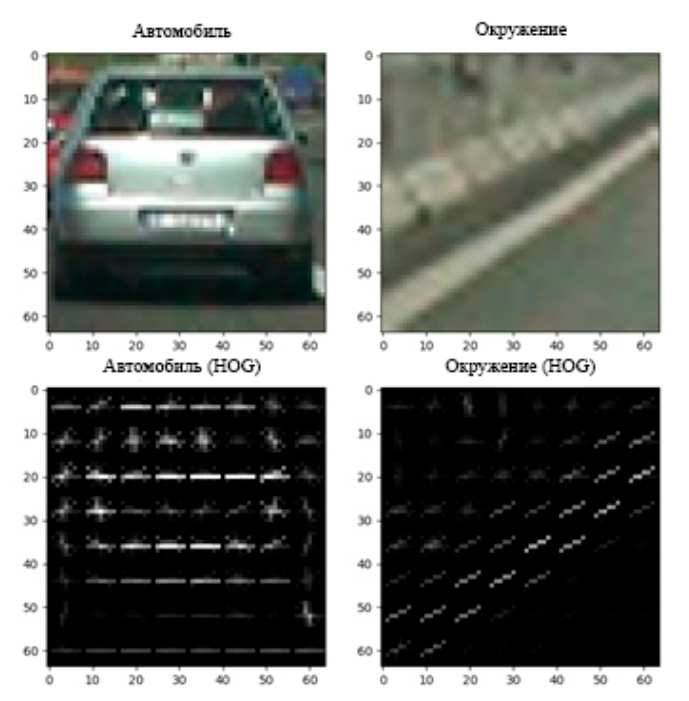
\includegraphics[width=0.5\textwidth]{image005.jpg}
\caption{Иллюстрация HOG-признаков~\cite{eight}}%
\label{fig:how-to-do-research}
\end{figure}

%%%%%%%%%%%%%%%%%%%%%%%%%%%%%%%%%%%%%%%%%%%%%%%%%%%%%%%%%%%%%%%%%%%%%%%%%%%%%%%%
\subsection{Классификация методом опорных веторов (Support Vector Machine)}
%%%%%%%%%%%%%%%%%%%%%%%%%%%%%%%%%%%%%%%%%%%%%%%%%%%%%%%%%%%%%%%%%%%%%%%%%%%%%%%%

Метод опорных векторов ~(SVM) — набор алгоритмов обучения с учителем, использующихся для задач классификации и регрессионного анализа. Принадлежит семейству линейных классификаторов. Особым свойством метода опорных векторов является непрерывное уменьшение эмпирической ошибки классификации и увеличение зазора, поэтому метод также известен как метод классификатора с максимальным зазором.
\nomenclature{SVM}{Support Vector Machine}

В алгоритмах машинного обучения возникает необходимость классифицировать данные. Каждый объект данных представляется как вектор (точка) в \(p\)-мерном пространстве (упорядоченный набор \(p\) чисел). Каждая из этих точек принадлежит только одному из двух классов. Вопрос состоит в том, можно ли разделить точки гиперплоскостью размерности \(p-1\). Это — типичный случай линейной разделимости. Искомых гиперплоскостей может быть много, поэтому полагают, что максимизация зазора между классами способствует более уверенной классификации. То есть, можно ли найти такую гиперплоскость, чтобы расстояние от неё до ближайшей точки было максимальным. Это эквивалентно тому, что сумма расстояний до гиперплоскости от двух ближайших к ней точек, лежащих по разные стороны от неё, максимальна. Если такая гиперплоскость существует, она называется оптимальной разделяющей гиперплоскостью, а соответствующий ей линейный классификатор называется оптимально разделяющим классификатором.

\begin{figure}[htbp]
\centering
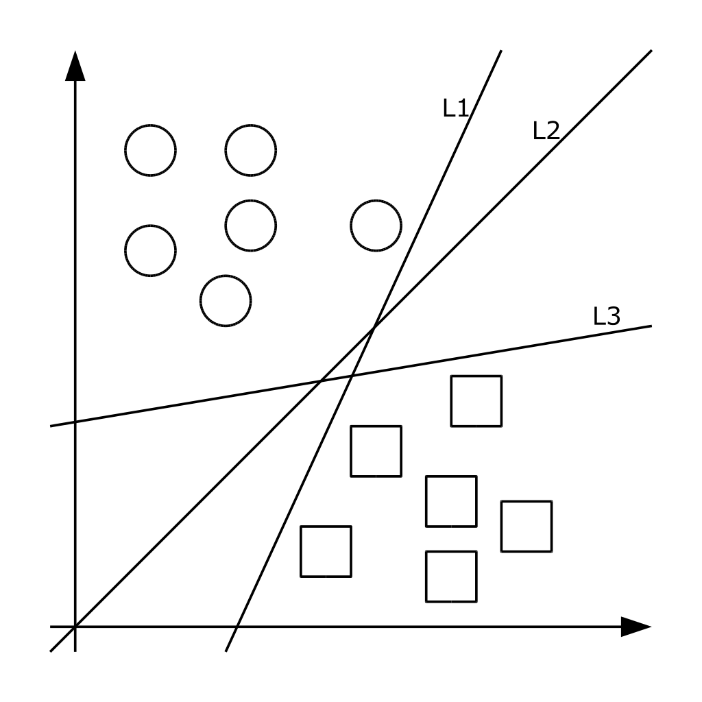
\includegraphics[width=0.5\textwidth]{image006.png}
\caption{Несколько классифицирующих разделяющих прямых (гиперплоскостей), из которых только одна соответствует оптимальному разделению~\cite{nine}}%
\label{fig:how-to-do-research}
\end{figure}

%%%%%%%%%%%%%%%%%%%%%%%%%%%%%%%%%%%%%%%%%%%%%%%%%%%%%%%%%%%%%%%%%%%%%%%%%%%%%%%%
\subsection{Обнаружение транспортных средств по частям (Part-based vehicle detection)}
%%%%%%%%%%%%%%%%%%%%%%%%%%%%%%%%%%%%%%%%%%%%%%%%%%%%%%%%%%%%%%%%%%%%%%%%%%%%%%%%

Обнаружение по частям используется чаще всего для ситуаций, где необходимо выполнить обнаружение транспортных средств в обстановке, где очень интенсивное движение. В таких ситуациях транспортные средства всегда скрыты большим количеством препятствий или другими участниками дорожного движения. В таких ситуациях методы, которые настроены на обнаружение целых транспортных средств не могут оперировать с высокой точностью. Для этого были разработаны специальные методы, которые позволяют определять признаки отдельных частей транспорта.

Транспортные средства сегментируются в соответствии с количеством частей, которые может определить алгоритм обнаружения. За определение каждой части транспортного средства отвечает отдельная часть алгоритма, каждая из которых настраивается отдельно. Для каждой части производится отдельное извлечение признака, как показано на рисунке ниже. После этого, результаты для каждой части сопоставляются вместе, чтобы предположить о нахождении целого транспортного средства. Процесс совмещения отдельных частей происходит на основе заранее определенных геометрических параметров. Однако работа такого алгоритма дает хорошие показатели в точности только тогда, когда имеется возможность обрабатывать кадры с высоким разрешением. 

\begin{figure}[htbp]
\centering
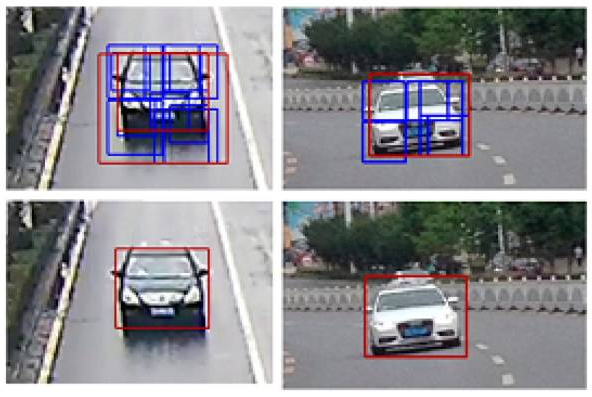
\includegraphics[width=0.5\textwidth]{image007.png}
\caption{Иллюстрация работы метода обнаружения по частям~\cite{ten}}%
\label{fig:how-to-do-research}
\end{figure}

%%%%%%%%%%%%%%%%%%%%%%%%%%%%%%%%%%%%%%%%%%%%%%%%%%%%%%%%%%%%%%%%%%%%%%%%%%%%%%%%
\section{Обнаружение транспортных средств с помощью обучаемых нейросетевых алгоритмов (Learning-Based Detection)}
%%%%%%%%%%%%%%%%%%%%%%%%%%%%%%%%%%%%%%%%%%%%%%%%%%%%%%%%%%%%%%%%%%%%%%%%%%%%%%%%

В основном, подобные алгоритмы основаны на нейронных сетях и требуют предварительного обучения на большом количестве примеров.

В представленной на рисунке ниже схеме даны основные, наиболее распространенные разновидности архитектур искусственных нейронных сетей.

\begin{figure}[htbp]
\centering
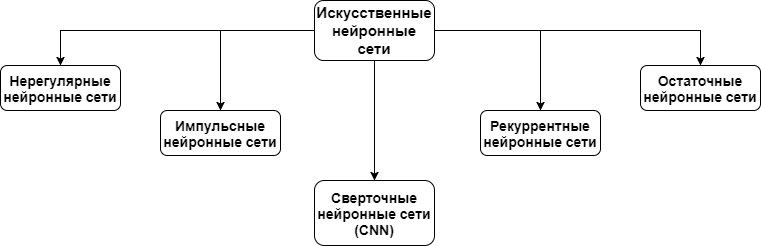
\includegraphics[width=\textwidth]{image008.png}
\caption{Основные архитектуры нейронных сетей}%
\label{fig:how-to-do-research}
\end{figure}

Конкретная разновидность архитектуры нейронной сети выбирается в зависимости от решаемой задачи. Среди наиболее часто используемых типов архитектур выделяют: нерегулярные нейронные сети, импульсные нейронные сети, сверточные нейронные сети, рекуррентные нейронные сети и остаточные нейронные сети. Сверточные нейронные сети являются наиболее часто используемой архитектурой при решении задач технического зрения.

Сверточные нейронные сети, также, как и обычные нейронные сети, состоят из нейронов с обучаемыми весами. Каждый нейрон получает на вход определенное значение, умножает его на весовой коэффициент и преобразует его через нелинейную функцию активации. Однако архитектура подобной сети строится из соображения что на вход подаются пиксели изображения, как показано на рисунке ниже. 

\begin{figure}[htbp]
\centering
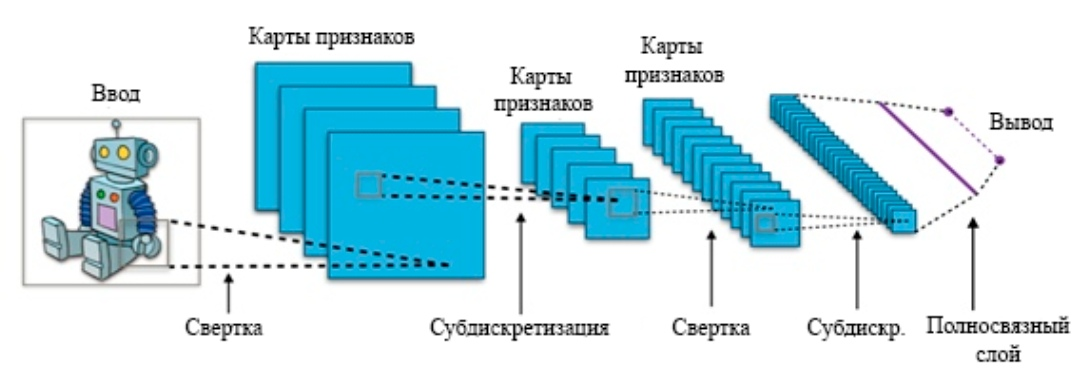
\includegraphics[width=\textwidth]{image009.jpg}
\caption{Архитектура сверточной нейронной сети~\cite{eleven}}%
\label{fig:how-to-do-research}
\end{figure}

Сверточная нейронная сеть характеризуется шириной, высотой и глубиной. Сеть состоит из последовательно расположеных слоёв нейронов, которые выполняют определенные функции. Используются следующие типы слоев и операции: слой свертки, операция субдискретизации и полносвязный слой. Архитектура сверточной нейронной сети строится из последовательно расположенных слоев и операций этих типов.

Сверточные слои реализуют алгебраическую операцию свертки двух матриц. Каждый сверточный слой имеет определенный набор параметров, которые называются фильтрами. Матрица, образованная сверточным слоем, используется для свертки входного изображения и построения карты признаков. Используя несколько фильтров, можно выделить различные признаки во входном изображении. Если последовательно расположить несколько слоев свертки, то можно выделить во входном изображении более высокоуровневые признаки.

Операция субдискретизации (англ. subsampling, англ. pooling, также переводимая как «операция подвыборки» или операция объединения), выполняет уменьшение размерности сформированных карт признаков. В данной архитектуре сети считается, что информация о факте наличия искомого признака важнее точного знания его координат, поэтому из нескольких соседних нейронов карты признаков выбирается максимальный и принимается за один нейрон уплотнённой карты признаков меньшей размерности. За счёт данной операции, помимо ускорения дальнейших вычислений, сеть становится более инвариантной к масштабу входного изображения.

Основная функция полносвязного слоя заключается в использовании построенной карты признаков для определения какому классу эту признаки соответствуют. Количество выходов полносвязного слоя зависит от количества классов, которые умеет обнаруживать данная нейронная сеть~\cite{twelve}.

%%%%%%%%%%%%%%%%%%%%%%%%%%%%%%%%%%%%%%%%%%%%%%%%%%%%%%%%%%%%%%%%%%%%%%%%%%%%%%%%
\subsection{YOLOv3 детектор}
%%%%%%%%%%%%%%%%%%%%%%%%%%%%%%%%%%%%%%%%%%%%%%%%%%%%%%%%%%%%%%%%%%%%%%%%%%%%%%%%

Данная сеть выдвигает гипотезы о четырех координатах для каждой области, где содержится объект. При обучении сети, с помощью этих координат вычисляется ошибка, на основе разницы гипотетических координат и исходных данных. Координаты гипотетической области определяются как те, которые наиболее точно перекрывают область с заданным объектом. Высота и ширина области гипотезы описываются как некоторые отступы от центроида кластера. Координаты центра рассчитываются относительно координат на выходе фильтра после применения к ним сигмоидальной функции.

Во время обучения используется квадратичная функция ошибки для оценки точности сети. В частности, для всех обучающих примеров находится разность между заданными координатами области и полученными на выходе детектора. Сеть также позволяет обрабатывать несколько гипотетических областей, из которых учитывается только та, которая наиболее точно перекрывает исходную область. Если какая-то из гипотез перекрывает заданную область несколько хуже другой гипотезы, то менее точная гипотеза не учитывается, даже если перекрытие области составило выше порогового. 

Каждый участок сетки может содержать области с объектами нескольких классов, что позволяет определять вложенные области, а также объекты пересекающихся классов (например «кошка» и «животное»). В ходе работы детектора гипотезы выдвигаются 3 раза. Таким образом, после получения выходного тензора, содержащего координаты и класс гипотезы, дополнительно используются карты признаков предыдущих слоев (признаки более низкого уровня), которые дополняются картами признаков слоев, идущих за ними. В результате данной операции размер выходного тензора увеличивается. Подобное комбинирование карт признаков с разных стадий свертки позволяет учитывать низкоуровневые признаки полученные на более ранних этапах свертки. 

\begin{figure}[htbp]
\centering
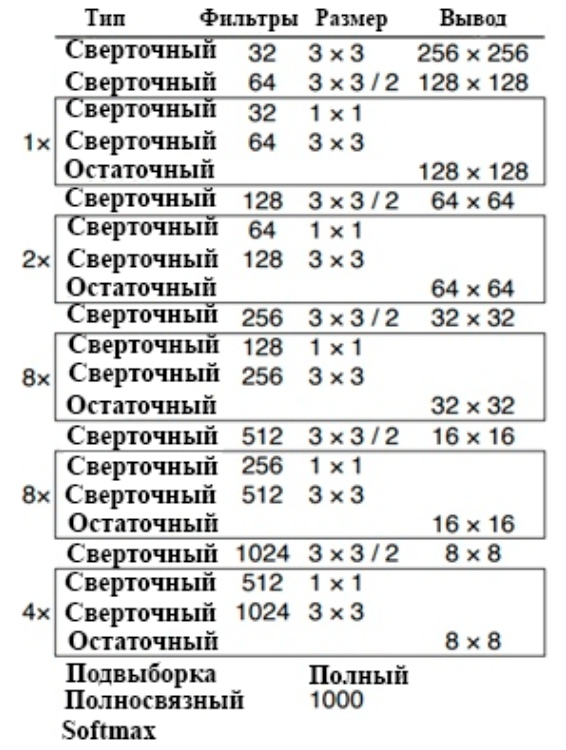
\includegraphics[width=0.5\textwidth]{image010.jpg}
\caption{Экстрактор признаков сети YOLOv3~\cite{thirteen}}%
\label{fig:how-to-do-research}
\end{figure}

Экстрактор признаков данной сети состоит из последовательных сверточных слоев, некоторые из которых соединены напрямую без учета порядка следования. Стоит отметить, что данная сеть имеет более высокое отношение операций с дробными числами к бинарным операциям, что позволяет больше вычислений производить на ~(GPU).
\nomenclature{GPU}{Graphics Processing Unit}
При минимальном пороге пересечения областей равном 0.5 YOLOv3 имеет относительно высокие показатели точности, однако при учете пересечений с коэффициентом больше 0.5 — точность заметно снижается, что позволяет сделать выводы о том, что возникают проблемы с точным выравниванием области гипотезы.

%%%%%%%%%%%%%%%%%%%%%%%%%%%%%%%%%%%%%%%%%%%%%%%%%%%%%%%%%%%%%%%%%%%%%%%%%%%%%%%%
\subsection{SSD детектор}
%%%%%%%%%%%%%%%%%%%%%%%%%%%%%%%%%%%%%%%%%%%%%%%%%%%%%%%%%%%%%%%%%%%%%%%%%%%%%%%%

\begin{table}
% Для таблиц с multirow и multicol необходимо вручную указать сдвиг для caption
\captionsetup{skip=5pt}
\caption{Example}
\centering
\begin{tabular}{|r|c|c|c|c|c|c|}
\hline
            \multirow{2}{*}{}
           & \multicolumn{2}{c|}{LLVM IR} 
           & \multicolumn{2}{c|}{PS} 
           & \multicolumn{2}{c|}{AI} \\ \cline{2-7}
           & SAT    & UNSAT   & SAT    & UNSAT   & SAT    & UNSAT   \\ \hline
beanstalkd & 356    & 252     & 360    & 161     & 360    & 247     \\ \hline
clib       & 599    & 258     & 960    & 234     & 960    & 449     \\ \hline
\end{tabular}
\label{table:checkResults}
\end{table}

%%%%%%%%%%%%%%%%%%%%%%%%%%%%%%%%%%%%%%%%%%%%%%%%%%%%%%%%%%%%%%%%%%%%%%%%%%%%%%%%
\section{bar}
%%%%%%%%%%%%%%%%%%%%%%%%%%%%%%%%%%%%%%%%%%%%%%%%%%%%%%%%%%%%%%%%%%%%%%%%%%%%%%%%

\blindtext
It is of great importance that you use correct references in your dissertation.
Resent studies show that it can increase the chances of successful defense
by as much as 3,17 percent~\cite{one}.

\begin{table}[H]
	\caption{Название таблицы}
	\begin{center}
		\begin{tabular}{|l|l|}
			\hline
			top left & top right\\ \hline
			bot left & bot right\\ \hline
		\end{tabular}
		\label{tabular:tab_examp}
	\end{center}
\end{table}


\Blindtext
